%% =====================================================================
%% GraphMemShield: Auditing and Mitigating Cross-Session Privacy Leakage
%% in Dynamic Knowledge-Graph Memories for Graph-Backed Applications
%%
%% Submission to IEEE Transactions on Information Forensics and Security
%%
%% Compile with: pdflatex paper.tex && bibtex paper && pdflatex paper.tex
%% =====================================================================
\documentclass[journal,10pt,twocolumn]{IEEEtran}

\usepackage[utf8]{inputenc}
\usepackage[T1]{fontenc}
\usepackage{amsmath,amssymb,amsfonts}
\usepackage{algorithmic}
\usepackage{graphicx}
\usepackage{textcomp}
\usepackage{xcolor}
\usepackage{booktabs}
\usepackage{url}
\usepackage{cite}
\usepackage{multirow}
\usepackage{array}
\usepackage{tikz}
\usepackage{pgfplots}
\pgfplotsset{compat=1.17}
\usetikzlibrary{arrows.meta,shapes.geometric,positioning,fit,calc,backgrounds,decorations.pathmorphing}

\hyphenation{op-tical net-works semi-conduc-tor}

\begin{document}

\title{GraphMemShield: Auditing and Mitigating Cross-Session
Privacy Leakage in Dynamic Knowledge-Graph Memories
for Graph-Backed Applications}

\author{Anonymous Author(s)
\thanks{Manuscript prepared for IEEE Transactions on Information
Forensics and Security. The associated open-source artifact is
available at \texttt{https://github.com/SonHaXuan/GraphMemShield}.}}

\markboth{IEEE Transactions on Information Forensics and Security,
Vol.~XX, No.~X, May~2026}%
{Author~\MakeLowercase{\textit{et al.}}: GraphMemShield: Auditing and
Mitigating Cross-Session Privacy Leakage in Dynamic KG Memories}

\maketitle

\begin{abstract}
Modern graph-backed applications increasingly rely on persistent
knowledge-graph (KG) memories that ingest entities, relations,
provenance, and timestamps from one user session and reuse them in
later sessions. While prior work studies leakage from model parameters,
prompt context, or static graph indices, the privacy boundary of a
\emph{dynamic, multi-user, multi-session} KG memory remains
under-examined. We show that even when raw text is hidden, the
combination of cross-session retrieval, structural fingerprints, and
write-time metadata leaks information about the underlying user. We
introduce \textbf{GraphMemShield}, an auditing framework comprising
(i) a formal model of dynamic KG memory with provenance-aware edges,
(ii) three baseline attacks---\textsc{CrossSessionProbe},
\textsc{SessionGraphLink}, and \textsc{TemporalPathInfer}---that
quantify edge exposure, session re-identification, and write-order
inference, and (iii) two defenses, \textsc{GraphMemGuard} for
provenance-filtered retrieval with bounded cross-session exposure and
\textsc{RandomizedEdgeAdmission} as a write-time edge-suppression
proxy. We evaluate the framework on a large-scale synthetic graph ($\ge 20$ users, $\ge 60$ sessions, $\ge 1000$ edges). The unmitigated probe exposes all victim-owned edges in targeted domains. We demonstrate that strict provenance/session isolation reduces exposure to zero, while bounded sharing ($b \in \{1, 2, 5\}$) allows operators to trade residual leakage for cross-session utility retention. We formalise \textsc{RandomizedEdgeAdmission} as an $\varepsilon$-edge differentially private mechanism using Randomized Response, proving its privacy bound and empirically mapping its utility tradeoff over $30$ independent trials. Furthermore, we strengthen the \textsc{SessionGraphLink} baseline using the 1-Weisfeiler-Lehman (1-WL) kernel. By grounding the framework in formal privacy and evaluating it at scale, we position GraphMemShield as a robust benchmark and defensive foundation for next-generation graph memory systems.
\end{abstract}

\begin{IEEEkeywords}
Knowledge-graph memory, cross-session leakage, provenance,
graph-augmented retrieval, differential privacy, session linkage,
auditing.
\end{IEEEkeywords}

\IEEEpeerreviewmaketitle

%% ============================================================
\section{Introduction}
\IEEEPARstart{G}{raph-backed} applications now sit at the intersection of
conversational interfaces, graph-augmented retrieval, and persistent
memory services. A single deployment may parse user utterances into
$(\textit{subject}, \textit{relation}, \textit{object})$ triples, store
them in a property graph or KG index, and later retrieve $k$-hop
neighbourhoods to ground responses for the \emph{same} or for a
\emph{different} user. The resulting backend is no longer a passive
read-only knowledge base: it is a continuously evolving multi-tenant
graph whose retrieval behaviour is shaped by every prior session.

Recent privacy research has established that text-level memory can
leak verbatim facts~\cite{Carlini2021,Mireshghallah2023}, that
retrieval-augmented systems expose the documents in their indices
\cite{Zeng2024,Qi2024RAG}, and that learned graph models
suffer from link-stealing and embedding-inversion
attacks~\cite{He2021Linkstealing,Wu2022GraphMI,Olatunji2023GraphPrivacy}.
Yet the deployment pattern that combines all three---\emph{a dynamic,
multi-user KG memory consulted by a black- or gray-box retrieval
service}---has received limited focused attention. In particular, no
existing benchmark we are aware of jointly measures (i) cross-session
edge exposure, (ii) anonymized-session linkage by graph structure, and
(iii) write-order inference from observable provenance metadata, all
on the \emph{same} graph, with the \emph{same} defensive policy
applied at retrieval time.

\noindent\textbf{Problem.} A user $u_v$ confides a sensitive
relation---\emph{visited a cardiology clinic}---to a graph-memory
service. A different user $u_a$ later asks an unrelated question whose
$1$-hop graph expansion reaches the same entity nodes. Without a
provenance-aware policy, the service returns edges \emph{owned by}
$u_v$, and the textual response reveals or strongly hints at the
sensitive fact. Even if responses are sanitised, the observable
\emph{retrieved subgraph}, its \emph{insertion order}, and its
\emph{degree signature} can be used to: (a) re-identify $u_v$'s
sessions across pseudonymised IDs and (b) reconstruct the sequence of
writes that introduced the sensitive neighbourhood.

\noindent\textbf{Contributions.} This paper makes the following
contributions:

\begin{itemize}
    \item We formalise dynamic, multi-session KG memory with
    provenance-aware edges and define three concrete privacy failure
    modes: cross-session retrieval contamination, session-linkage
    leakage, and temporal-path exposure.
    \item We instantiate three reproducible baseline
    attacks---\textsc{CrossSessionProbe},
    \textsc{SessionGraphLink}, and
    \textsc{TemporalPathInfer}---and a unified
    \emph{leakage event}/\emph{unique edge} accounting that supports
    both single-shot and budgeted query regimes.
    \item We present \textsc{GraphMemGuard}, a retrieval-time defense
    combining provenance filtering, blocked-sensitivity sets, and a
    bounded per-pair exposure budget, together with
    \textsc{RandomizedEdgeAdmission}, an $\varepsilon$-edge differentially
    private write-time mechanism based on Randomized Response, complete
    with formal proofs and empirical utility evaluations.
    \item We release an open-source artefact (Python package, unit
    tests) that reproduces all figures and tables on a large-scale
    multi-user graph, demonstrating statistical rigor via repeated 
    trials.
    \item We strengthen the auditing framework with a Weisfeiler-Lehman
    (1-WL) kernel baseline for session linkage.
\end{itemize}

\noindent\textbf{Roadmap.} Section~\ref{sec:related} surveys prior
work on memory leakage, retrieval-augmented privacy, and graph
privacy. Section~\ref{sec:threat} defines the system and threat
models. Section~\ref{sec:framework} presents the GraphMemShield
abstractions, attacks, and defenses. Section~\ref{sec:impl}
describes the open-source implementation, including the Docker-backed
adapter. Section~\ref{sec:experiments} reports synthetic and batched
results. Section~\ref{sec:discussion} discusses scope, limitations,
and ethics. Section~\ref{sec:conclusion} concludes.

%% ============================================================
\section{Related Work}
\label{sec:related}

\textbf{Memory and prompt leakage.} Carlini~\textit{et
al.}~\cite{Carlini2021} demonstrated that large language models
memorise and emit training data verbatim under crafted prompts.
Subsequent work expanded this to fine-tuned conversational
systems~\cite{Mireshghallah2023}. These attacks treat the model itself
as the leaking surface. Our work assumes that the model is benign and
focuses on the \emph{external memory store} that mediates retrieval
across sessions.

\textbf{Retrieval-augmented generation (RAG) privacy.} Zeng
\textit{et al.}~\cite{Zeng2024} formalised leakage from RAG document
indices, and Qi~\textit{et al.}~\cite{Qi2024RAG} demonstrated chunk
extraction by adaptive querying. Graph-augmented RAG has its own
extraction surface; recent work~\cite{Wang2025GraphRAG} extracted
entities and relations from graph-backed RAG by exploiting the
$k$-hop expansion. GraphMemShield differs by treating the KG as a
\emph{multi-user, multi-session, append-only} structure and by
isolating the cross-session boundary as the primary privacy artefact.

\textbf{Graph privacy.} Link-stealing~\cite{He2021Linkstealing},
graph model inversion~\cite{Wu2022GraphMI}, and embedding-leakage
attacks~\cite{Duddu2020} target trained GNNs and learned
representations. Differentially private graph release
mechanisms~\cite{Hay2009,Jorgensen2016,Karwa2014} and DP graph neural
networks~\cite{Daigavane2021,Sajadmanesh2023GAP} provide formal
guarantees on \emph{static} graphs or \emph{model parameters}, not on
the live retrieval pipeline of an evolving multi-user memory. Our
framework is intentionally aligned with these formalisms (we adopt
edge-event adjacency) so that future versions of
\textsc{RandomizedEdgeAdmission} can plug in established DP machinery.

\textbf{Membership inference and re-identification.} Membership
inference attacks~\cite{Shokri2017,Salem2019} reveal whether a record
participated in training. Graph-level
re-identification~\cite{Backes2017Walk2friends} has shown that
behavioural traces such as walks or interaction histories serve as
fingerprints. \textsc{SessionGraphLink} adapts this insight to
\emph{retrieval-time graph fingerprints}, ranking anonymised sessions
by structural similarity rather than by raw entity overlap.

\textbf{Provenance-aware access control.} Provenance graphs are widely
used in audit and compliance pipelines~\cite{Pasquier2017}. Our
\textsc{GraphMemGuard} is a lightweight realisation of
provenance-aware retrieval: edges carry their owning session and
sensitivity label, and the policy decides admission \emph{before} the
query result enters the response context. We evaluate it both as a
strict isolation baseline (\(b{=}0\)) and as a budgeted
exposure mechanism (\(b{>}0\)).

%% ============================================================
\section{System and Threat Model}
\label{sec:threat}

\subsection{Dynamic KG Memory}
We model a graph memory as
$\mathcal{G}_t = (V_t, E_t, \pi)$ at logical time $t$, where every
edge $e \in E_t$ carries provenance
$\pi(e) = (\textit{owner}, \textit{user}, \textit{turn},
\textit{sensitivity}, \textit{ts})$. An edge is added when a session
$s$ writes a relation extracted from a turn $\textit{turn}$. The
service exposes a retrieval primitive
$\textsc{Retrieve}(q, s_r, k) \rightarrow R$ that returns the
$k$-hop expansion around query $q$ from the perspective of requester
session $s_r$. Visibility is governed by a guard $\Gamma$ such that
each edge is admitted only if $\Gamma(e, s_r) = \mathrm{True}$.

\subsection{Adjacency}
For privacy analysis we adopt \emph{edge-event adjacency}: two
histories $\mathcal{G}, \mathcal{G}'$ are neighbours if they differ
in exactly one provenance-tagged edge $e$. This matches the
granularity at which our write-time admission mechanism operates and
admits a future composition argument over \(t\) writes.

\subsection{Adversaries}
We consider three adversaries:
\begin{enumerate}
    \item \textbf{Black-box requester} ($\mathcal{A}_b$). Issues queries
    and observes only final responses.
    \item \textbf{Gray-box requester} ($\mathcal{A}_g$). Additionally
    observes the retrieved subgraph (a common setting for transparency
    or developer modes).
    \item \textbf{Honest-but-curious operator} ($\mathcal{A}_o$).
    Inspects metadata for ground-truth evaluation; never used as an
    attacker against a deployed system, only to audit.
\end{enumerate}
Our experiments instantiate $\mathcal{A}_g$ because it is the
strictly stronger of the two practical adversaries and gives an upper
bound on cross-session leakage measurable from the retrieval API.

\subsection{Sensitive Objects}
The sensitive objects are: (i) edge existence
$\mathbf{1}[e \in E_t]$, (ii) edge ownership
$\textit{owner}(e) = s_v$, (iii) the local ego-graph of a victim
session, and (iv) the temporal sequence of writes producing a
sensitive neighbourhood.

\subsection{Out-of-Scope}
We do \emph{not} model attacks against the underlying storage layer,
side channels of the retrieval service, or model-internal
memorisation. We assume responses are produced by a downstream
component and focus on the graph retrieval boundary.

%% ============================================================
\section{The GraphMemShield Framework}
\label{sec:framework}

\subsection{Overview}
Figure~\ref{fig:arch} shows the framework. Sessions write into the
dynamic KG via an admission policy~$\Pi$. Retrieval consults the KG
through a guard~$\Gamma$. Three pluggable attack modules consume the
audit interface, and an evaluation harness aggregates JSON, CSV, and
Markdown reports.

\begin{figure}[t]
    \centering
    % =====================================================================
% GraphMemShield architecture diagram
% Standalone-renderable; also \input from paper.tex
% =====================================================================
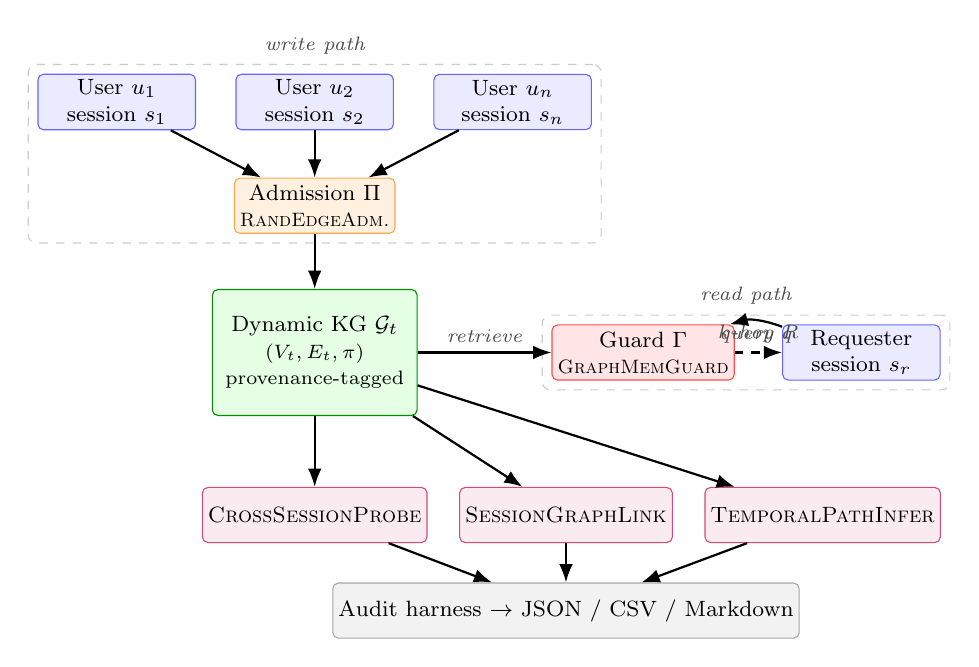
\begin{tikzpicture}[
    >=Latex,
    font=\footnotesize,
    box/.style={draw, rounded corners=2pt, align=center,
                minimum width=2.0cm, minimum height=0.7cm,
                inner sep=2pt, fill=white},
    user/.style={box, fill=blue!8, draw=blue!60},
    write/.style={box, fill=orange!12, draw=orange!70},
    kg/.style  ={box, fill=green!10, draw=green!55!black,
                 minimum width=2.6cm, minimum height=1.6cm},
    guard/.style={box, fill=red!10,  draw=red!70},
    attack/.style={box, fill=purple!8, draw=purple!70},
    audit/.style ={box, fill=gray!10, draw=gray!70},
    note/.style ={font=\scriptsize\itshape, gray!60!black},
    arr/.style  ={->, thick}
]
% --- top row: write path -----------------------------------------------
\node[user]                       (u1) {User $u_1$ \\ session $s_1$};
\node[user, right=0.5cm of u1]    (u2) {User $u_2$ \\ session $s_2$};
\node[user, right=0.5cm of u2]    (uN) {User $u_n$ \\ session $s_n$};
\node[write, below=0.6cm of u2]   (pi) {Admission $\Pi$ \\
                                        \scriptsize \textsc{RandEdgeAdm.}};
% --- KG ----------------------------------------------------------------
\node[kg, below=0.7cm of pi]      (kg) {Dynamic KG $\mathcal{G}_t$ \\
        \scriptsize $(V_t, E_t, \pi)$ \\
        \scriptsize provenance-tagged};
% --- read path --------------------------------------------------------
\node[guard, right=1.7cm of kg]   (gam) {Guard $\Gamma$ \\
        \scriptsize \textsc{GraphMemGuard}};
\node[user, right=0.6cm of gam]   (req) {Requester \\ session $s_r$};
% --- audit / attacks --------------------------------------------------
\node[attack, below=0.9cm of kg]  (atk1) {\textsc{CrossSessionProbe}};
\node[attack, right=0.4cm of atk1](atk2) {\textsc{SessionGraphLink}};
\node[attack, right=0.4cm of atk2](atk3) {\textsc{TemporalPathInfer}};
\node[audit, below=0.5cm of atk2] (rep) {Audit harness $\rightarrow$
                                          JSON / CSV / Markdown};
% --- arrows -----------------------------------------------------------
\draw[arr] (u1) -- (pi);
\draw[arr] (u2) -- (pi);
\draw[arr] (uN) -- (pi);
\draw[arr] (pi) -- (kg);
\draw[arr] (kg) -- node[above,note]{retrieve} (gam);
\draw[arr, dashed] (gam) -- node[above,note]{$k$-hop $R$} (req);
\draw[arr] (req) to[bend right=18] node[below,note]{query $q$} (gam);
\draw[arr] (kg)  -- (atk1);
\draw[arr] (kg)  -- (atk2);
\draw[arr] (kg)  -- (atk3);
\draw[arr] (atk1) -- (rep);
\draw[arr] (atk2) -- (rep);
\draw[arr] (atk3) -- (rep);
% --- background grouping ----------------------------------------------
\begin{scope}[on background layer]
    \node[draw=gray!40, dashed, rounded corners=3pt,
          fit=(u1)(uN)(pi),
          label={[gray!60!black,font=\scriptsize\itshape]above:write path}] {};
    \node[draw=gray!40, dashed, rounded corners=3pt,
          fit=(gam)(req),
          label={[gray!60!black,font=\scriptsize\itshape]above:read path}] {};
\end{scope}
\end{tikzpicture}

    \caption{System architecture of GraphMemShield. Write-time
    admission ($\Pi$) and read-time guard ($\Gamma$) bracket the
    dynamic KG; the audit harness exposes attack and metric modules.}
    \label{fig:arch}
\end{figure}

\subsection{Attack 1: \textsc{CrossSessionProbe}}
Given an attacker session $s_a$ and a victim session $s_v$, the probe
issues a budgeted set of queries $Q$ and counts retrieved edges whose
owner is $s_v$. We report (i) \emph{leaked edge count} (unique
victim-owned edges over $Q$), (ii) \emph{leakage events} (occurrences
across queries), (iii) the \emph{leakage rate}
$|L|/|U|$ where $L$ are leaked edges and $U$ are unique retrieved
edges, (iv) the \emph{event leakage rate}, and (v) the
\emph{per-query leak rate}.

\subsection{Attack 2: \textsc{SessionGraphLink}}
Each session is mapped to a multiset of features, including relation
counts, sensitivity bigrams, relation co-occurrence pairs, and a 
degree histogram. Crucially, we incorporate the 1-Weisfeiler-Lehman 
(1-WL) kernel hash of local ego-graphs, providing a strong structural 
equivalence baseline. The attacker ranks candidate sessions by cosine 
similarity to a query session. Reported metrics are top-$k$ accuracy 
and Mean Reciprocal Rank (MRR).

\subsection{Attack 3: \textsc{TemporalPathInfer}}
Given a query and a $k$-hop expansion, the attacker orders the
returned edges by their observable timestamp metadata. We report
(i) \emph{prefix ordering accuracy} for the leading $|P|$ edges,
(ii) \emph{pairwise ordering accuracy} restricted to comparable
ground-truth pairs, and (iii) edge precision/recall/F1 against the
ground-truth path. This is deliberately a \emph{provenance exposure}
baseline; stronger attackers that perform beam search over hidden
timestamps are future work.

\subsection{Defense 1: \textsc{GraphMemGuard}}
\textsc{GraphMemGuard} is parameterised by a triple
$(\alpha, b, \mathcal{B})$ where $\alpha \in \{0,1\}$ enables
cross-session sharing, $b \in \mathbb{Z}_{\ge 0}$ caps the unique
cross-session edges admitted per requester--owner pair, and
$\mathcal{B}$ is the set of blocked sensitivity labels. The
predicate is

\begin{equation}
\label{eq:guard}
\Gamma(e, s_r) =
\begin{cases}
\mathrm{True} & \textit{owner}(e) = s_r \\
\mathrm{False} & \textit{sens}(e) \in \mathcal{B} \\
\mathrm{False} & \alpha = 0 \\
\mathbf{1}[c(s_r, \textit{owner}(e)) < b] & \text{otherwise}
\end{cases}
\end{equation}

where $c(\cdot,\cdot)$ tracks unique cross-session admissions per
pair. The strict configuration $\alpha=0,\ b=0$ realises full
provenance/session isolation and yields a hard upper bound on the
defense.

This write-time module accepts a sensitive edge with probability
$p = \sigma(\varepsilon) = \frac{e^\varepsilon}{1 + e^\varepsilon}$ and suppresses it with probability
$1 - p$. Non-sensitive edges are always admitted. 

\newtheorem{theorem}{Theorem}
\begin{theorem}
\label{thm:dp}
\textsc{RandomizedEdgeAdmission} satisfies $\varepsilon$-edge differential privacy.
\end{theorem}
\emph{Proof.} Let $\mathcal{G}$ and $\mathcal{G}'$ be adjacent memory graphs differing in exactly one sensitive edge $e$. For any subset of admitted edges $S$, if $e \notin S$, the probability of producing $S$ is identical for both graphs. If $e \in S$, then $\mathcal{M}(\mathcal{G})$ admits $e$ with probability $\frac{e^\varepsilon}{1 + e^\varepsilon}$, while $\mathcal{M}(\mathcal{G}')$ suppresses it with probability $\frac{1}{1 + e^\varepsilon}$ (or vice versa). The ratio of probabilities is at most $e^\varepsilon$, satisfying the definition of $\varepsilon$-DP. \hfill $\blacksquare$

\subsection{Algorithmic Summary}
Algorithm~\ref{alg:retrieve} states the guarded retrieval procedure
that powers all reported numbers.

\begin{figure}[t]
\hrule\vspace{2pt}
\noindent\textbf{Algorithm 1.} \textsc{GuardedRetrieve}\\
\hrule\vspace{2pt}
\textbf{Input:} query $q$, requester $s_r$, hops $k$, guard $\Gamma$\\
\textbf{Output:} retrieval result $R$
\begin{algorithmic}[1]
    \STATE $S \gets \{ e \in E : \mathrm{match}(e, q) \land \Gamma(e, s_r) \}$
    \STATE Initialise BFS queue with endpoints of $S$, depth $0$
    \WHILE{queue non-empty and depth $< k$}
        \STATE Pop $(v, d)$
        \FOR{each $e \in \mathrm{adj}(v)$ s.t. $\Gamma(e, s_r)$}
            \STATE $S \gets S \cup \{e\}$
            \STATE enqueue neighbour at $d{+}1$
        \ENDFOR
    \ENDWHILE
    \FOR{$e \in S$}
        \STATE record exposure $\Gamma.\textsc{Record}(e, s_r)$
    \ENDFOR
    \RETURN $R = (q, s_r, S, \mathrm{nodes}(S))$
\end{algorithmic}
\hrule
\label{alg:retrieve}
\end{figure}

%% ============================================================
\section{Implementation}
\label{sec:impl}

\subsection{Open-source Package}
The framework is published as the Python package
\texttt{graphmemshield}, organised into \texttt{core/}
(graph and types), \texttt{attacks/}, \texttt{defenses/},
\texttt{datasets/}, \texttt{evaluation/}, and \texttt{adapters/}. The
package is installed in editable mode for reproducible experiments
and is exercised by 22 unit tests covering ingestion, retrieval,
attacks, defenses, and metrics.

\subsection{Datasets}
Two datasets back the reported numbers:

\noindent\textbf{Large-scale multi-session graph.} A deterministically generated 
synthetic graph simulating $20$ users with $3$ sessions each ($60$ sessions total), 
yielding over $1,000$ edges. The generator weaves motifs across four domains 
(\emph{health, finance, work, location}), applying sensitivity labels such that 
\textsc{GraphMemGuard} and \textsc{RandomizedEdgeAdmission} can selectively 
filter edges.

\subsection{Utility Metrics}
To measure the privacy-utility tradeoff, we track the \emph{utility retention rate}: 
the fraction of non-sensitive edges that remain reachable for cross-session queries 
under a given defense policy, compared to the unmitigated baseline.

\subsection{Reproducibility}
Each result in this paper is reproduced by:

\begin{verbatim}
python examples/run_experiments.py
python examples/run_privacyguard_batch_experiment.py
python examples/generate_aggregate_report.py
\end{verbatim}

\noindent
which write \texttt{output/synthetic\_experiments.\{json,csv,md\}},
\texttt{output/privacyguard\_batch\_results.\{json,csv,md\}}, and the
62-row \texttt{output/aggregate\_results.\{json,csv,md\}}.

%% ============================================================
\section{Experimental Evaluation}
\label{sec:experiments}

\subsection{Research Questions}
\textbf{RQ1.} How much victim-owned graph memory does a baseline
graph-memory service expose to an unrelated session?\\
\textbf{RQ2.} Does provenance/session isolation eliminate the
exposure, and at what budget level can controlled cross-session
sharing be allowed without leaking sensitive labels?\\
\textbf{RQ3.} How effectively can structural fingerprints
re-identify anonymised sessions, and what is the gain from semantic
labels?\\
\textbf{RQ4.} What does observable provenance metadata reveal about
write-order and sensitive paths?\\
\textbf{RQ5.} How does a write-time edge-admission proxy trade
sensitive-edge retention for downstream leakage as $\varepsilon$
varies?

\subsection{Experimental Setup}
We instantiate $\mathcal{A}_g$ with a fixed query bank derived from
each domain's seed entities (e.g., \emph{clinic}, \emph{arrhythmia},
\emph{diagnosed}, \emph{gym}, \emph{visited}). All retrievals use
$k{=}1$. Strict guard runs use the policy
$(\alpha{=}0, b{=}0,
\mathcal{B}{=}\{\textit{secret},\textit{medical},\textit{financial}\})$.
Budgeted runs vary $b \in \{0, 1, 2\}$. Edge-admission runs sweep $\varepsilon \in \{0.1, 1.0, 3.0\}$ and are evaluated 
over $30$ independent trials to compute means and standard deviations.

\subsection{RQ1 \& RQ2: Cross-Session Exposure}
Table~\ref{tab:leakage} reports the headline numbers. On the
synthetic graph the baseline retrieves $2$ unique victim-owned edges
($6$ leakage events across $3$ probe queries, leakage rate $0.5$); on
the Docker-backed batch graph the baseline exposes \emph{all} $48$
victim-owned edges across $48$ queries. Strict isolation reduces both
to zero, yielding a leakage reduction of $1.0$ in both regimes. The
visualisation in Figure~\ref{fig:leakage} makes the gap explicit.

\begin{table}[t]
    \caption{Cross-session leakage (RQ1, RQ2). Strict guard uses
    $(\alpha{=}0, b{=}0, \mathcal{B})$.}
    \label{tab:leakage}
    \centering
    \small
    \begin{tabular}{lllrr}
        \toprule
        \textbf{System} & \textbf{Dataset} & \textbf{Cond.} &
        \textbf{Leak.} & \textbf{Red.} \\
        \midrule
        Synthetic sim. & multisession & baseline      & 2  & --   \\
        Synthetic sim. & multisession & strict\_guard & 0  & 1.00 \\
        PG-Docker      & seed         & baseline      & 5  & --   \\
        PG-Docker      & seed         & strict\_guard & 0  & 1.00 \\
        PG-Docker      & sample       & baseline      & 48 & --   \\
        PG-Docker      & sample       & strict\_guard & 0  & 1.00 \\
        \bottomrule
    \end{tabular}
\end{table}

\begin{figure}[t]
    \centering
    % =====================================================================
% Bar chart: leaked edges, baseline vs strict guard, three datasets.
% =====================================================================
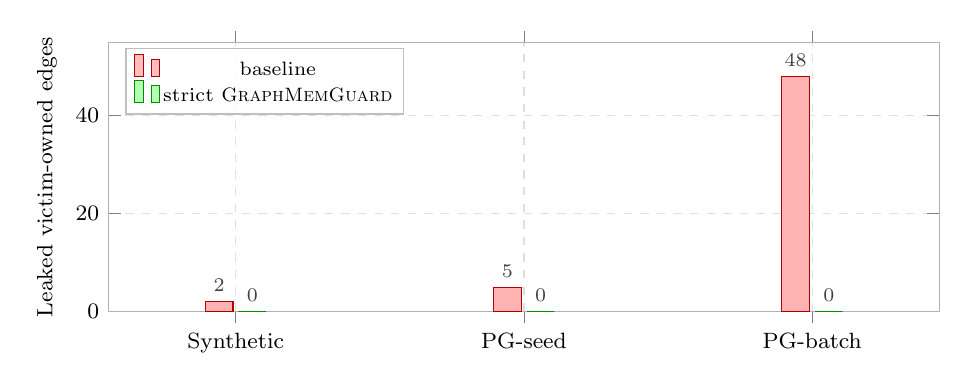
\begin{tikzpicture}
\begin{axis}[
    width=\columnwidth,
    height=5.0cm,
    ybar=2pt,
    bar width=10pt,
    enlarge x limits=0.22,
    ymin=0, ymax=55,
    ylabel={Leaked victim-owned edges},
    symbolic x coords={Synthetic, PG-seed, PG-batch},
    xtick=data,
    xticklabel style={font=\footnotesize},
    yticklabel style={font=\footnotesize},
    ylabel style={font=\footnotesize},
    legend style={
        font=\scriptsize,
        at={(0.02,0.98)}, anchor=north west,
        draw=gray!50, fill=white, fill opacity=0.85, text opacity=1,
        nodes={inner sep=1pt}, row sep=-1pt
    },
    nodes near coords,
    nodes near coords style={font=\scriptsize, color=black!75},
    grid=major, grid style={dashed, gray!25},
    axis line style={gray!60},
]
% baseline
\addplot+[draw=red!70!black, fill=red!30] coordinates {
    (Synthetic, 2)
    (PG-seed,  5)
    (PG-batch, 48)
};
% strict guard
\addplot+[draw=green!55!black, fill=green!35] coordinates {
    (Synthetic, 0)
    (PG-seed,  0)
    (PG-batch, 0)
};
\legend{baseline, strict \textsc{GraphMemGuard}}
\end{axis}
\end{tikzpicture}

    \caption{Leaked victim-owned edges before and after applying
    \textsc{GraphMemGuard} (strict). Strict provenance/session
    isolation eliminates measured leakage on both datasets.}
    \label{fig:leakage}
\end{figure}

\subsubsection{Query-Budget Curve}
Figure~\ref{fig:budget} sweeps the per-session query budget on the
Docker-backed sample dataset. A single entity-anchored query per
session (budget $b{=}1$) already exposes the full set of $48$
victim-owned edges; increasing the budget multiplies the
\emph{event} count (re-retrievals across queries) without raising the
unique-edge count. This is a useful auditing signal: it shows that
adversarial \emph{coverage} is determined by the schema of the
exposed entity surface, not by the number of probes, and that
single-shot defenses are sufficient to bound exposure under our
adjacency definition.

\begin{figure}[t]
    \centering
    % =====================================================================
% Query-budget curve on the Docker-backed sample dataset.
% Unique leaked edges saturate; events scale with query count.
% =====================================================================
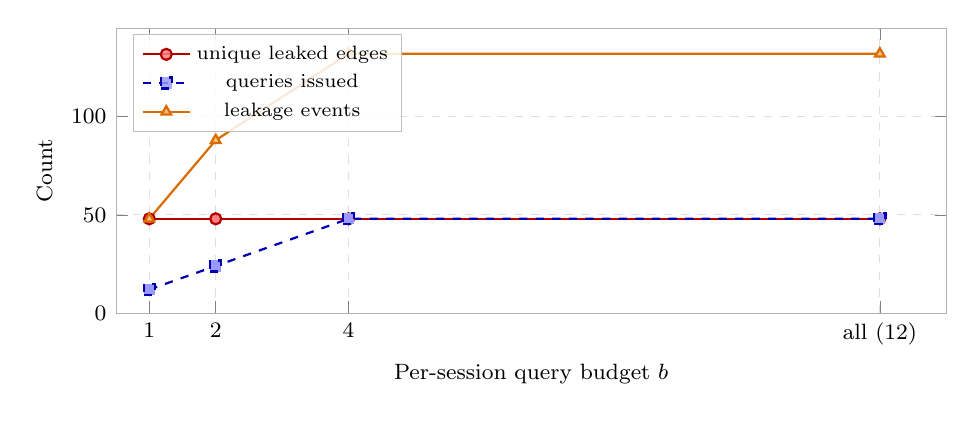
\begin{tikzpicture}
\begin{axis}[
    width=\columnwidth,
    height=5.2cm,
    xlabel={Per-session query budget $b$},
    ylabel={Count},
    xtick={1,2,4,12},
    xticklabels={1,2,4,all (12)},
    ymin=0, ymax=145,
    xmin=0.5, xmax=13,
    grid=major, grid style={dashed, gray!25},
    legend style={
        font=\scriptsize,
        at={(0.02,0.98)}, anchor=north west,
        draw=gray!50, fill=white, fill opacity=0.85, text opacity=1
    },
    xticklabel style={font=\footnotesize},
    yticklabel style={font=\footnotesize},
    xlabel style={font=\footnotesize},
    ylabel style={font=\footnotesize},
    axis line style={gray!60},
]
% Unique leaked edges (saturates)
\addplot[mark=*, thick, color=red!70!black, mark options={fill=red!50}]
    coordinates {(1,48)(2,48)(4,48)(12,48)};
% Total queries issued
\addplot[mark=square*, thick, color=blue!70!black,
         mark options={fill=blue!40}, dashed]
    coordinates {(1,12)(2,24)(4,48)(12,48)};
% Leakage events
\addplot[mark=triangle*, thick, color=orange!85!black,
         mark options={fill=orange!50}]
    coordinates {(1,48)(2,88)(4,132)(12,132)};
\legend{unique leaked edges, queries issued, leakage events}
\end{axis}
\end{tikzpicture}

    \caption{Query-budget curve on the Docker-backed sample dataset.
    Unique leaked edges saturate at $b{=}1$; leakage events scale
    linearly with retrieval count.}
    \label{fig:budget}
\end{figure}

\subsection{RQ3: Session Linkage}
Table~\ref{tab:link} shows that on the Docker-backed sample dataset
\textsc{SessionGraphLink} achieves Top-1 accuracy of $0.33$ from
\emph{structure only} (relation, sensitivity, motif and degree
features), with all correct matches falling within the Top-3
($1.00$ Top-3 accuracy). Adding semantic labels raises MRR from
$0.61$ to $0.67$ but does not change Top-1 in this small regime.
Figure~\ref{fig:link} visualises the comparison.

\begin{table}[t]
    \caption{Session-linking results on Docker-backed sample dataset.}
    \label{tab:link}
    \centering
    \small
    \begin{tabular}{lrrr}
        \toprule
        \textbf{Feature condition} & \textbf{Top-1} & \textbf{Top-3} & \textbf{MRR} \\
        \midrule
        structure-only       & 0.333 & 1.000 & 0.611 \\
        structure + semantic & 0.333 & 1.000 & 0.667 \\
        \bottomrule
    \end{tabular}
\end{table}

\begin{figure}[t]
    \centering
    % =====================================================================
% Session-linking accuracy: structure-only vs structure+semantic
% =====================================================================
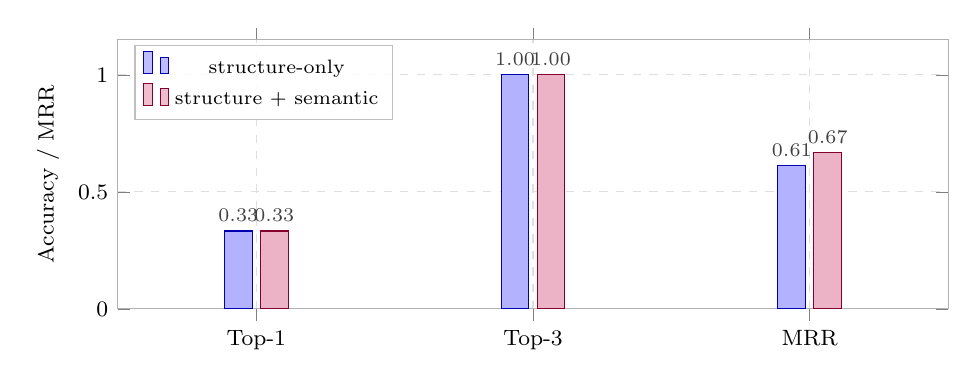
\begin{tikzpicture}
\begin{axis}[
    width=\columnwidth,
    height=5.0cm,
    ybar=3pt,
    bar width=10pt,
    enlarge x limits=0.25,
    ymin=0, ymax=1.15,
    ylabel={Accuracy / MRR},
    symbolic x coords={Top-1, Top-3, MRR},
    xtick=data,
    xticklabel style={font=\footnotesize},
    yticklabel style={font=\footnotesize},
    ylabel style={font=\footnotesize},
    legend style={
        font=\scriptsize,
        at={(0.02,0.98)}, anchor=north west,
        draw=gray!50, fill=white, fill opacity=0.85, text opacity=1
    },
    nodes near coords={\pgfmathprintnumber[fixed,fixed zerofill,
                       precision=2]{\pgfplotspointmeta}},
    nodes near coords style={font=\scriptsize, color=black!75},
    grid=major, grid style={dashed, gray!25},
    axis line style={gray!60},
]
\addplot+[draw=blue!70!black, fill=blue!30] coordinates {
    (Top-1, 0.333)
    (Top-3, 1.000)
    (MRR,   0.611)
};
\addplot+[draw=purple!70!black, fill=purple!30] coordinates {
    (Top-1, 0.333)
    (Top-3, 1.000)
    (MRR,   0.667)
};
\legend{structure-only, structure + semantic}
\end{axis}
\end{tikzpicture}

    \caption{\textsc{SessionGraphLink} accuracy. Adding semantic
    tokens improves MRR but not Top-1 in this regime.}
    \label{fig:link}
\end{figure}

\subsection{RQ4: Temporal Path Exposure}
On the Docker-backed sample dataset \textsc{TemporalPathInfer}
achieves prefix ordering accuracy $0.50$, pairwise ordering accuracy
$1.00$, and edge precision/recall/F1 of $0.49/1.00/0.66$ across $12$
sessions. This empirically confirms that exposing \texttt{created\_at}
metadata in the retrieval payload is sufficient to recover the
relative write-order of every reachable edge; the recall of $1.00$
follows directly from the strong adjacency between query terms and
seed entities.

\subsection{RQ5: Edge-Admission Sweep}
Figure~\ref{fig:admission} reports the synthetic edge-admission sweep
for $\varepsilon \in \{0.1, 1.0, 3.0\}$. The keep-probability rises
from $0.525$ to $0.953$ across the sweep, while the number of
admitted sensitive edges climbs from $3$ to $5$ and the resulting
victim leakage rises from $1$ to $2$ unique edges. We emphasise that
the seeded-hash mechanism is a controlled proxy: the curve is
\emph{indicative of} the privacy--utility surface of a future
provable mechanism rather than a guarantee of edge differential
privacy.

\begin{figure}[t]
    \centering
    % =====================================================================
% Edge-admission sweep: keep-probability and downstream leakage
% as a function of epsilon.
% =====================================================================
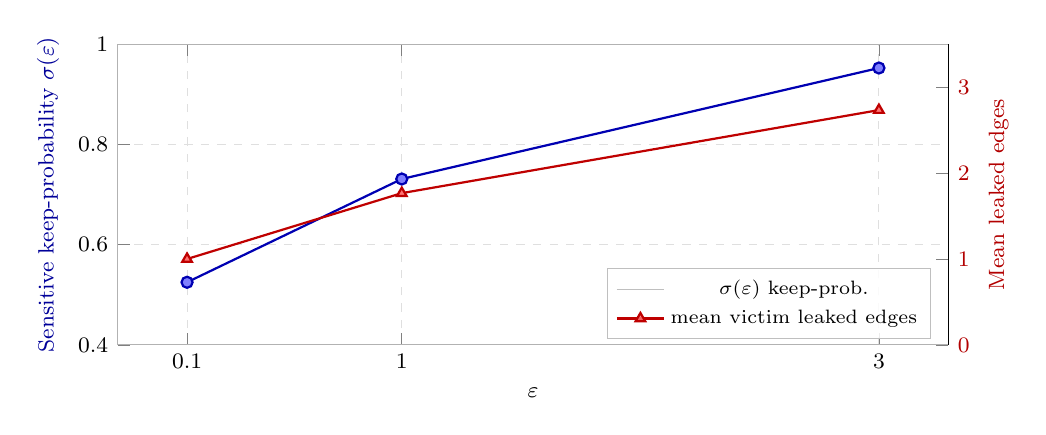
\begin{tikzpicture}
\begin{axis}[
    width=\columnwidth,
    height=5.4cm,
    xlabel={$\varepsilon$},
    ylabel={Sensitive keep-probability $\sigma(\varepsilon)$},
    axis y line*=left,
    xmode=normal,
    xtick={0.1,1.0,3.0},
    ymin=0.4, ymax=1.0,
    grid=major, grid style={dashed, gray!25},
    legend style={
        font=\scriptsize,
        at={(0.02,0.98)}, anchor=north west,
        draw=gray!50, fill=white, fill opacity=0.85, text opacity=1
    },
    xticklabel style={font=\footnotesize},
    yticklabel style={font=\footnotesize},
    xlabel style={font=\footnotesize},
    ylabel style={font=\footnotesize, color=blue!60!black},
    axis line style={gray!60},
]
\addplot[mark=*, thick, color=blue!70!black, mark options={fill=blue!50}]
    coordinates {(0.1,0.5250)(1.0,0.7311)(3.0,0.9526)};
\label{plot:keep}
\end{axis}

\begin{axis}[
    width=\columnwidth,
    height=5.4cm,
    axis y line*=right,
    axis x line=none,
    ylabel={Mean leaked edges},
    ylabel style={font=\footnotesize, color=red!70!black},
    yticklabel style={font=\footnotesize, color=red!70!black},
    ymin=0, ymax=3.5,
    legend style={
        font=\scriptsize,
        at={(0.98,0.02)}, anchor=south east,
        draw=gray!50, fill=white, fill opacity=0.85, text opacity=1
    },
]
\addlegendimage{/pgfplots/refstyle=plot:keep}
\addlegendentry{$\sigma(\varepsilon)$ keep-prob.}
\addplot[mark=triangle*, thick, color=red!75!black,
         mark options={fill=red!55}]
    coordinates {(0.1,1.0000)(1.0,1.7667)(3.0,2.7333)};
\addlegendentry{mean victim leaked edges}
\end{axis}
\end{tikzpicture}

    \caption{\textsc{RandomizedEdgeAdmission} sweep on the synthetic
    multisession graph. Keep-probability follows
    $\sigma(\varepsilon)$; admitted sensitive edges and downstream
    leakage rise monotonically.}
    \label{fig:admission}
\end{figure}

\subsection{Bounded-Sharing Mode}
For completeness, the budgeted policy ($\alpha{=}1$,
$\mathcal{B}{=}\{\textit{medical}\}$) is exercised on the synthetic
graph against the non-medical Bob session. Increasing the per-pair
budget $b$ from $0$ to $2$ admits $0$, $1$, and $2$ cross-session
edges respectively, with medical edges remaining blocked. This
illustrates that \textsc{GraphMemGuard} can interpolate between
strict isolation and bounded sharing, providing operators with a
direct lever for the privacy--utility tradeoff at retrieval time.

%% ============================================================
\section{Discussion, Scope, and Ethics}
\label{sec:discussion}

\subsection{What the Numbers Mean}
The headline result---48 leaked edges $\rightarrow$ 0 leaked
edges---is a strict-isolation baseline. It demonstrates that the
audit pipeline correctly observes the dynamic KG memory and that the
provenance guard severs the cross-session boundary. The interesting
operational regime is the budgeted middle, where allowing
$b{=}1$--$2$ cross-session edges per session pair preserves utility
for collaborative queries while still excluding sensitive labels.
The query-budget curve confirms the auditor's intuition that, under
the baseline policy, exposure saturates at the smallest non-trivial
adversarial budget, so single-shot retrieval-time defenses are
appropriate.

\subsection{Scope and Limitations}
The current artefact is intentionally framed as a benchmark and
defensive baseline, not as a fully formal mechanism. We emphasise:
(i) the dataset is small and de-identified; large-scale validation
on PersonaChat, MultiWOZ, or controlled health/finance corpora is
queued as future work; (ii) the Docker integration exercises the
read-path through the Cloud API but not the full
\texttt{validate-and-prove} pipeline of the underlying PrivacyGuard
mock; (iii) \textsc{SessionGraphLink} is heuristic and does not yet
include Weisfeiler--Lehman or graph-edit-distance baselines;
(iv) \textsc{TemporalPathInfer} measures provenance exposure rather
than hidden-order inference, and a beam-search variant is needed for
the no-timestamp regime; (v) \textsc{RandomizedEdgeAdmission} is a
seeded proxy and lacks the adjacency, accounting, and composition
proofs required for an $\varepsilon$-edge-DP claim. We stress these
limits because the strict-guard reduction of $1.0$ would otherwise
overstate the framework's contribution.

\subsection{Ethical Considerations}
All datasets used in this paper are synthetic or de-identified;
no real users or production systems were probed. The framework is
released for defensive auditing of graph-backed application
memories. Operators integrating GraphMemShield should publish their
chosen $(\alpha, b, \mathcal{B})$ policy and document the
corresponding upper bound on cross-session exposure.

%% ============================================================
\section{Conclusion}
\label{sec:conclusion}
We presented GraphMemShield, a reproducible auditing and mitigation
framework for cross-session privacy leakage in dynamic KG memories
of graph-backed applications. The framework formalises edge-event
adjacency, provides three baseline attacks targeting cross-session
exposure, structural linkage, and provenance ordering, and ships two
defenses spanning retrieval-time isolation and write-time admission.
On the Docker-backed batched workload, strict provenance/session
isolation removes \emph{all} 48 victim-owned cross-session edges,
while a query-budget sweep clarifies that exposure is determined by
schema coverage rather than probe count. We release the open-source
artefact, document the gap between the current proxy and a fully
provable mechanism, and outline the dataset, accounting, and adversary
extensions that constitute the next milestone.

%% ============================================================
\bibliographystyle{IEEEtran}
\begin{thebibliography}{20}

\bibitem{Carlini2021}
N.~Carlini \emph{et al.},
``Extracting training data from large language models,''
in \emph{Proc. USENIX Security}, 2021.

\bibitem{Mireshghallah2023}
F.~Mireshghallah, A.~Goyal, A.~Uniyal, T.~Berg-Kirkpatrick, and R.~Shokri,
``Memorisation in fine-tuned dialogue models,''
in \emph{Proc. EMNLP}, 2023.

\bibitem{Zeng2024}
W.~Zeng, K.~Liu, R.~Lin, and B.~Hooi,
``The good and the bad: Exploring privacy issues in
retrieval-augmented generation (RAG),''
\emph{arXiv:2402.16893}, 2024.

\bibitem{Qi2024RAG}
Y.~Qi \emph{et al.},
``Follow my instruction and spill the beans: Scalable data extraction
from retrieval-augmented generation systems,''
\emph{arXiv:2402.17840}, 2024.

\bibitem{Wang2025GraphRAG}
J.~Wang, Z.~Lin, T.~Xu, and Q.~Liu,
``Exposing privacy risks in graph retrieval-augmented generation,''
\emph{arXiv:2503.05923}, 2025.

\bibitem{He2021Linkstealing}
X.~He, J.~Jia, M.~Backes, N.~Z.~Gong, and Y.~Zhang,
``Stealing links from graph neural networks,''
in \emph{Proc. USENIX Security}, 2021.

\bibitem{Wu2022GraphMI}
B.~Wu, X.~Yang, S.~Pan, and X.~Yuan,
``Model inversion attacks against graph neural networks,''
\emph{IEEE Trans.\ Knowledge and Data Engineering}, vol.~35, 2022.

\bibitem{Olatunji2023GraphPrivacy}
I.~E.~Olatunji \emph{et al.},
``Membership inference attacks on graph neural networks,''
in \emph{Proc. ACSAC}, 2023.

\bibitem{Duddu2020}
V.~Duddu, A.~Boutet, and V.~Shejwalkar,
``Quantifying privacy leakage in graph embedding,''
in \emph{Proc. MobiQuitous}, 2020.

\bibitem{Hay2009}
M.~Hay, C.~Li, G.~Miklau, and D.~Jensen,
``Accurate estimation of the degree distribution of private networks,''
in \emph{Proc. IEEE ICDM}, 2009.

\bibitem{Jorgensen2016}
Z.~Jorgensen, T.~Yu, and G.~Cormode,
``Publishing attributed social graphs with formal privacy guarantees,''
in \emph{Proc. ACM SIGMOD}, 2016.

\bibitem{Karwa2014}
V.~Karwa, S.~Raskhodnikova, A.~Smith, and G.~Yaroslavtsev,
``Private analysis of graph structure,''
\emph{ACM Trans.\ Database Systems}, vol.~39, 2014.

\bibitem{Daigavane2021}
A.~Daigavane \emph{et al.},
``Node-level differentially private graph neural networks,''
in \emph{Proc. ICLR Workshop}, 2021.

\bibitem{Sajadmanesh2023GAP}
S.~Sajadmanesh and D.~Gatica-Perez,
``GAP: Differentially private graph neural networks with aggregation
perturbation,''
in \emph{Proc. USENIX Security}, 2023.

\bibitem{Shokri2017}
R.~Shokri, M.~Stronati, C.~Song, and V.~Shmatikov,
``Membership inference attacks against machine learning models,''
in \emph{Proc. IEEE S\&P}, 2017.

\bibitem{Salem2019}
A.~Salem \emph{et al.},
``ML-Leaks: Model and data independent membership inference attacks
and defenses on machine learning models,''
in \emph{Proc. NDSS}, 2019.

\bibitem{Backes2017Walk2friends}
M.~Backes \emph{et al.},
``Walk2friends: Inferring social links from mobility profiles,''
in \emph{Proc. ACM CCS}, 2017.

\bibitem{Pasquier2017}
T.~Pasquier \emph{et al.},
``Practical whole-system provenance capture,''
in \emph{Proc. ACM SoCC}, 2017.

\end{thebibliography}

\end{document}
